%\subsection{تخمین پارامترهای کانال پیچ موتور خاموش}
%برای اصلاح پارامترهای پیچ چندین آزمایش انجام شد و با استفاده از داده‌های ثبت شده از وضعیت استند در کانال پیچ و جعبه‌ابزار
%\lr{Parameter Estimator}،
%پارامترهای کانال پیچ اصلاح شدند.
%برای انجام آزمایش استند از شرایط اولیه مختلف با موتور خاموش رها شد  و از خروجی سنسور داده برداری شد. سپس، مدل و داده‌های ثبت شده‌ی سنسور (وضعیت استند در کانال پیچ) به جعبه‌ابزار
%\lr{Parameter Estimator}
%داده‌شد. وضعیت کانال پیچ استند در شبیه‌سازی و واقعیت بعد از اصلاح پارامترهای کانال پیچ در شکل‌های
%\ref{pitch_ml_ps1}, \ref{pitch_ml_ps3} , \ref{pitch_ml_ps4}  و \ref{pitch_ml_ps5}
%مقایسه شده است.
%
%\begin{figure}[H]
%	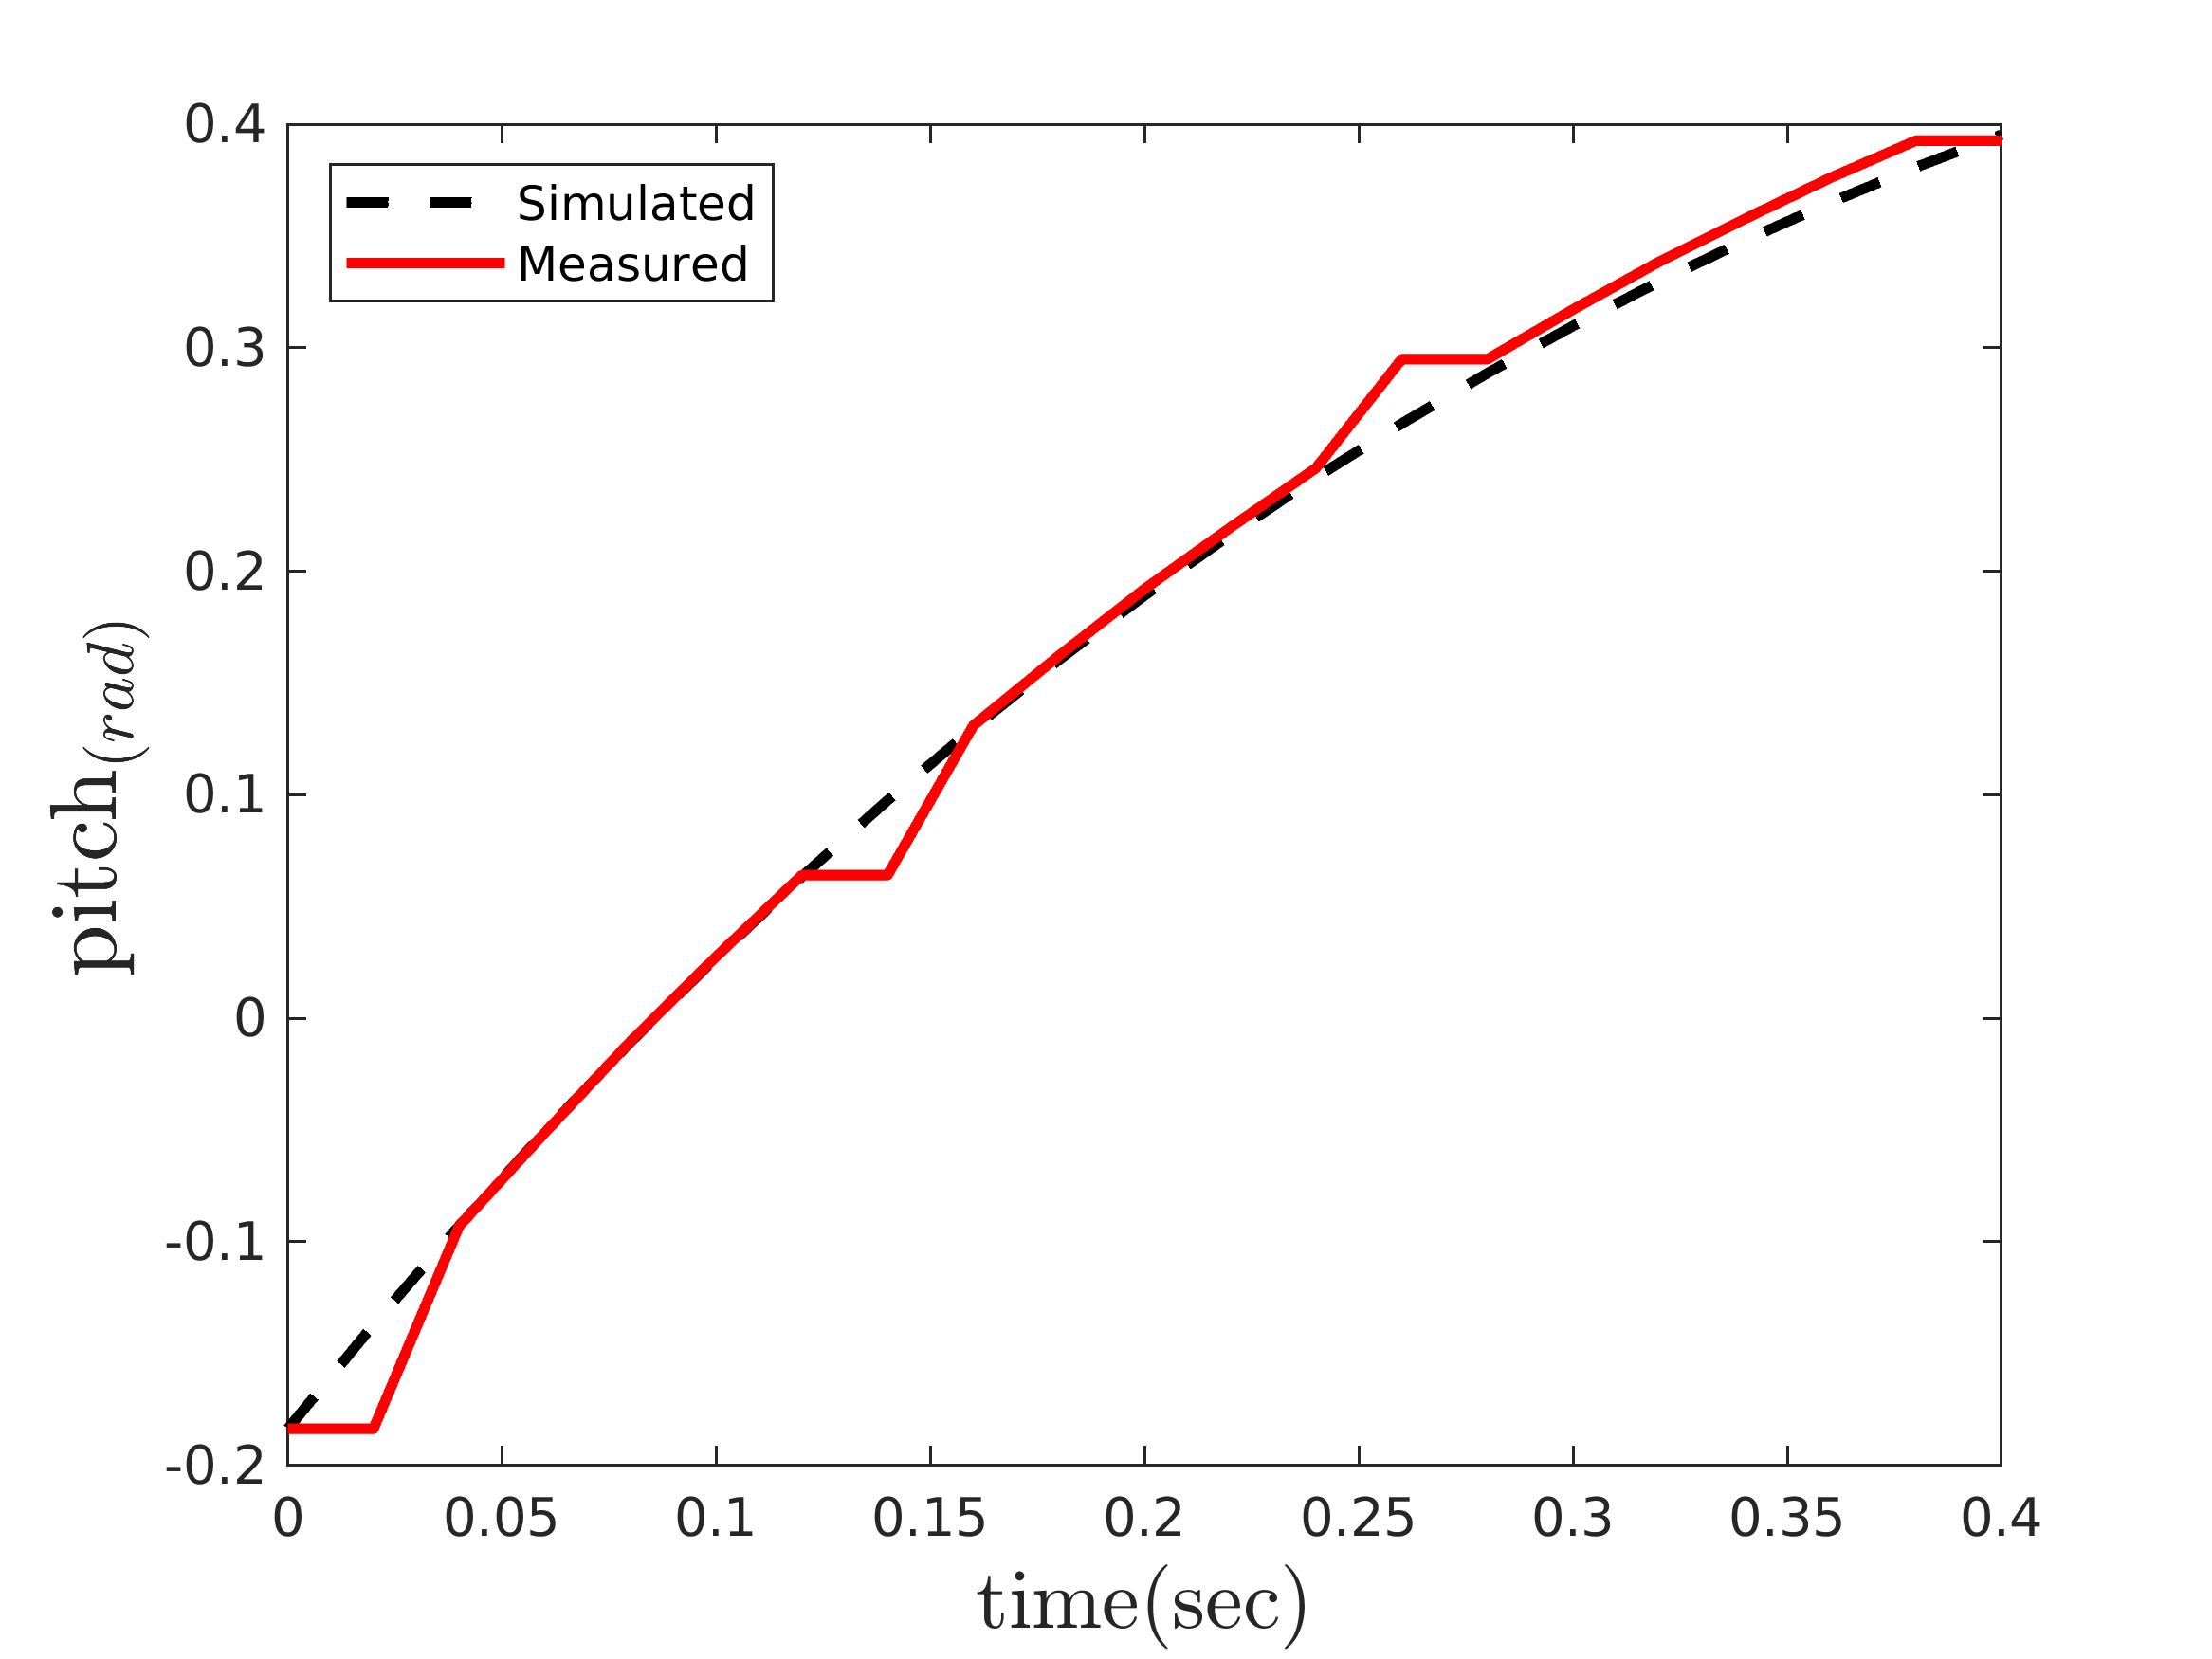
\includegraphics[width=.48\linewidth]{../Figures/RCP/pitch_ml_parameter_estimation/RCP_pitch_S1.png}
%	\centering
%	\caption{مقايسه وضعیت استند در  آزمايش اول و شبیه‌سازی، پس از تخمین پارامترهای کانال پیچ موتور خاموش}
%	\label{pitch_ml_ps1}
%\end{figure}
%\begin{figure}[H]
%	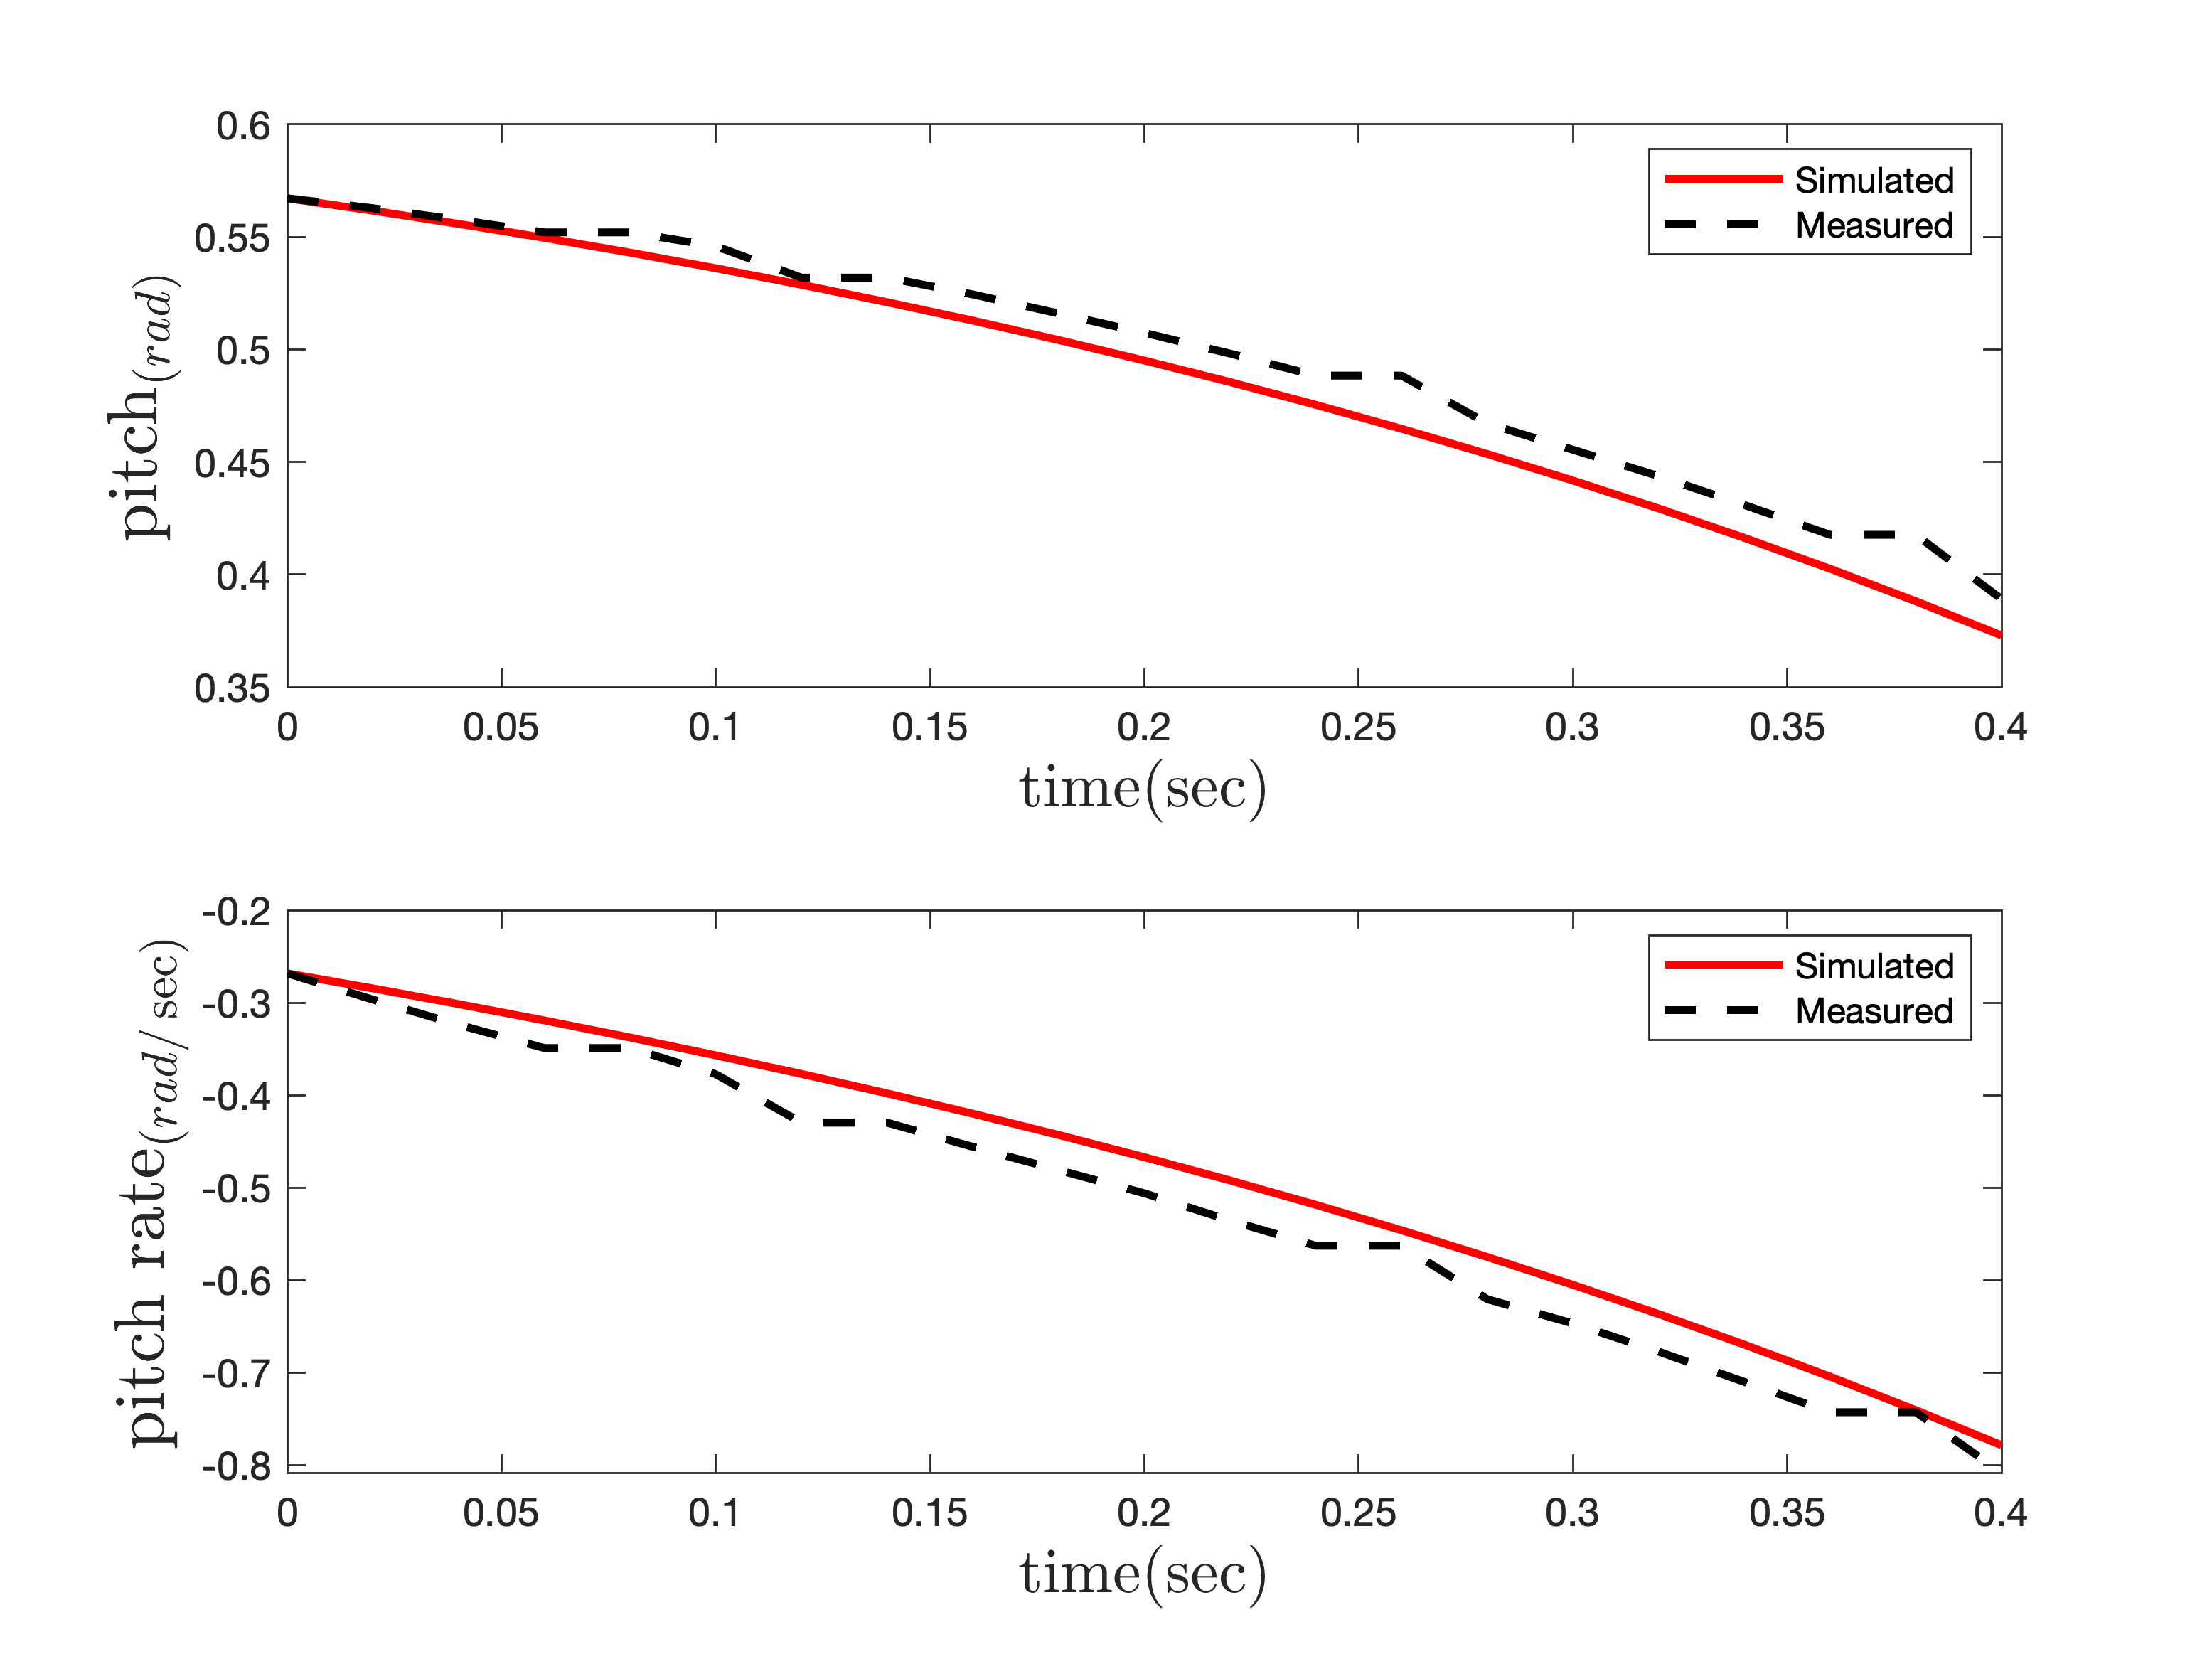
\includegraphics[width=12cm]{../Figures/RCP/pitch_ml_parameter_estimation/RCP_pitch_S2.png}
%	\centering
%	\caption{مقايسه وضعیت استند در  آزمايش دوم و شبیه‌سازی، پس از تخمین پارامترهای کانال پیچ موتور خاموش}
%	\label{pitch_ml_ps2}
%\end{figure}
%\begin{figure}[H]
%	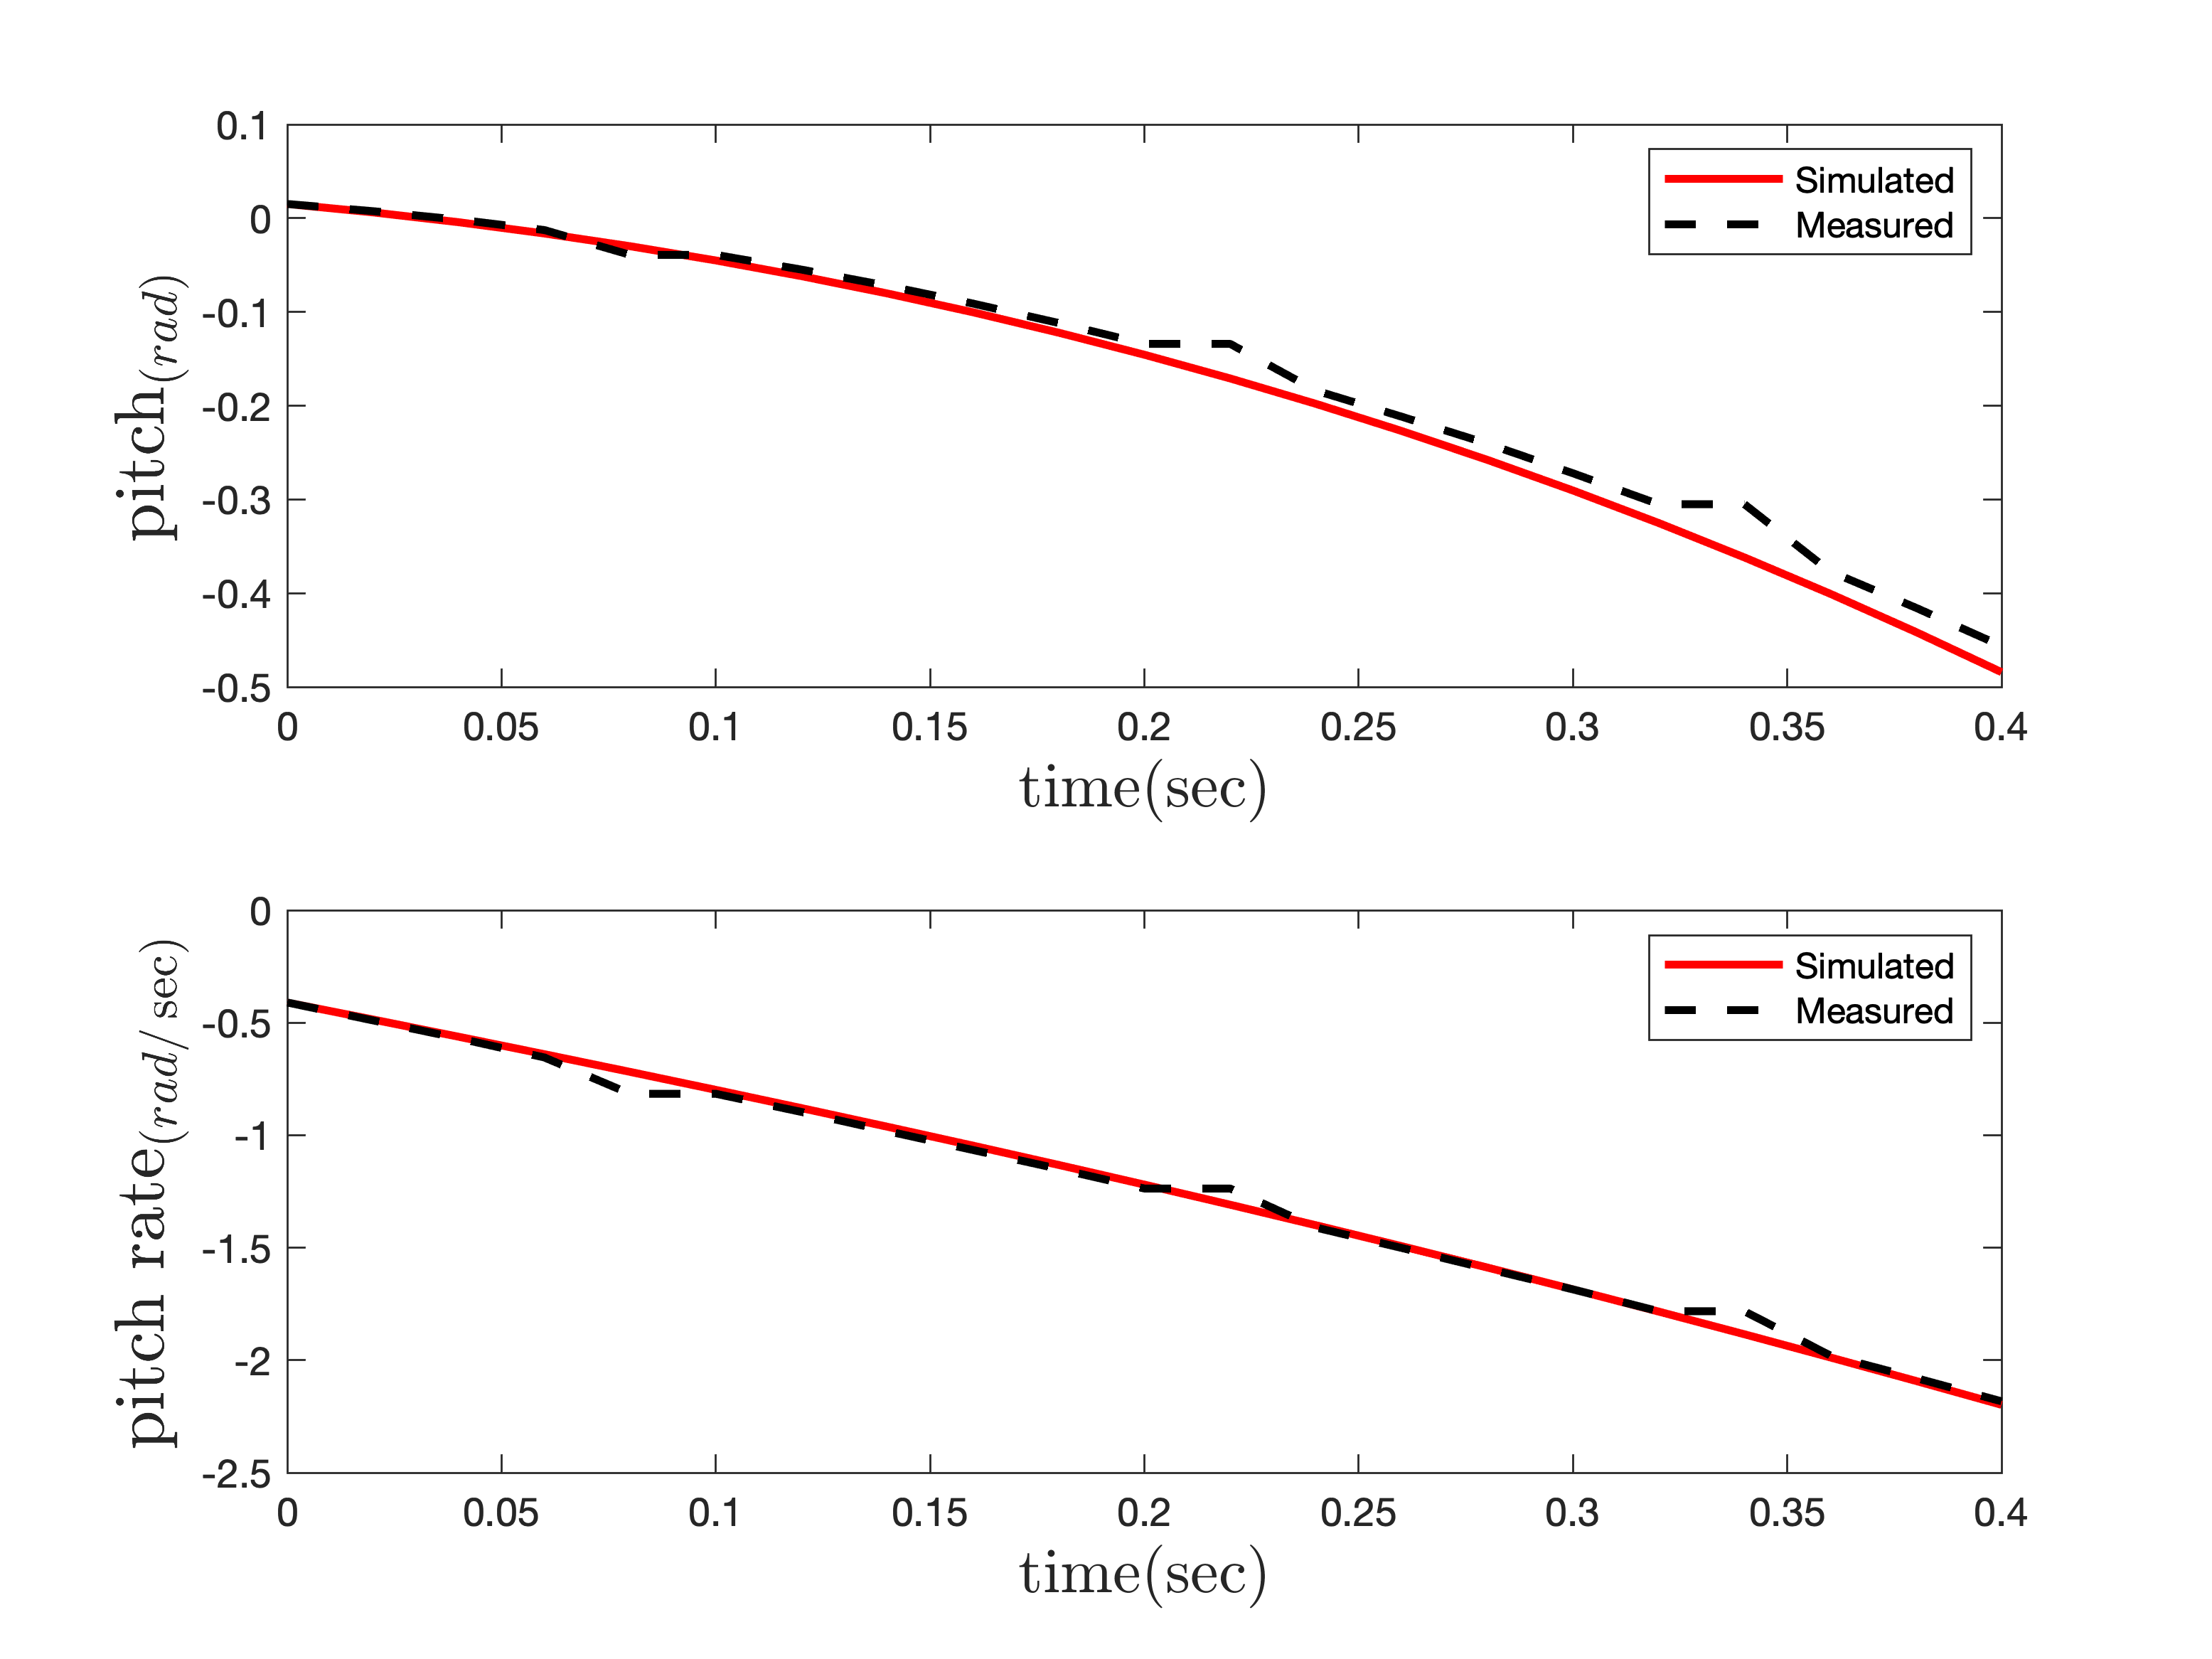
\includegraphics[width=12cm]{../Figures/RCP/pitch_ml_parameter_estimation/RCP_pitch_S3.png}
%	\centering
%	\caption{مقايسه وضعیت استند در  آزمايش سوم و شبیه‌سازی، پس از تخمین پارامترهای کانال پیچ موتور خاموش}
%	\label{pitch_ml_ps3}
%\end{figure}
%\begin{figure}[H]
%	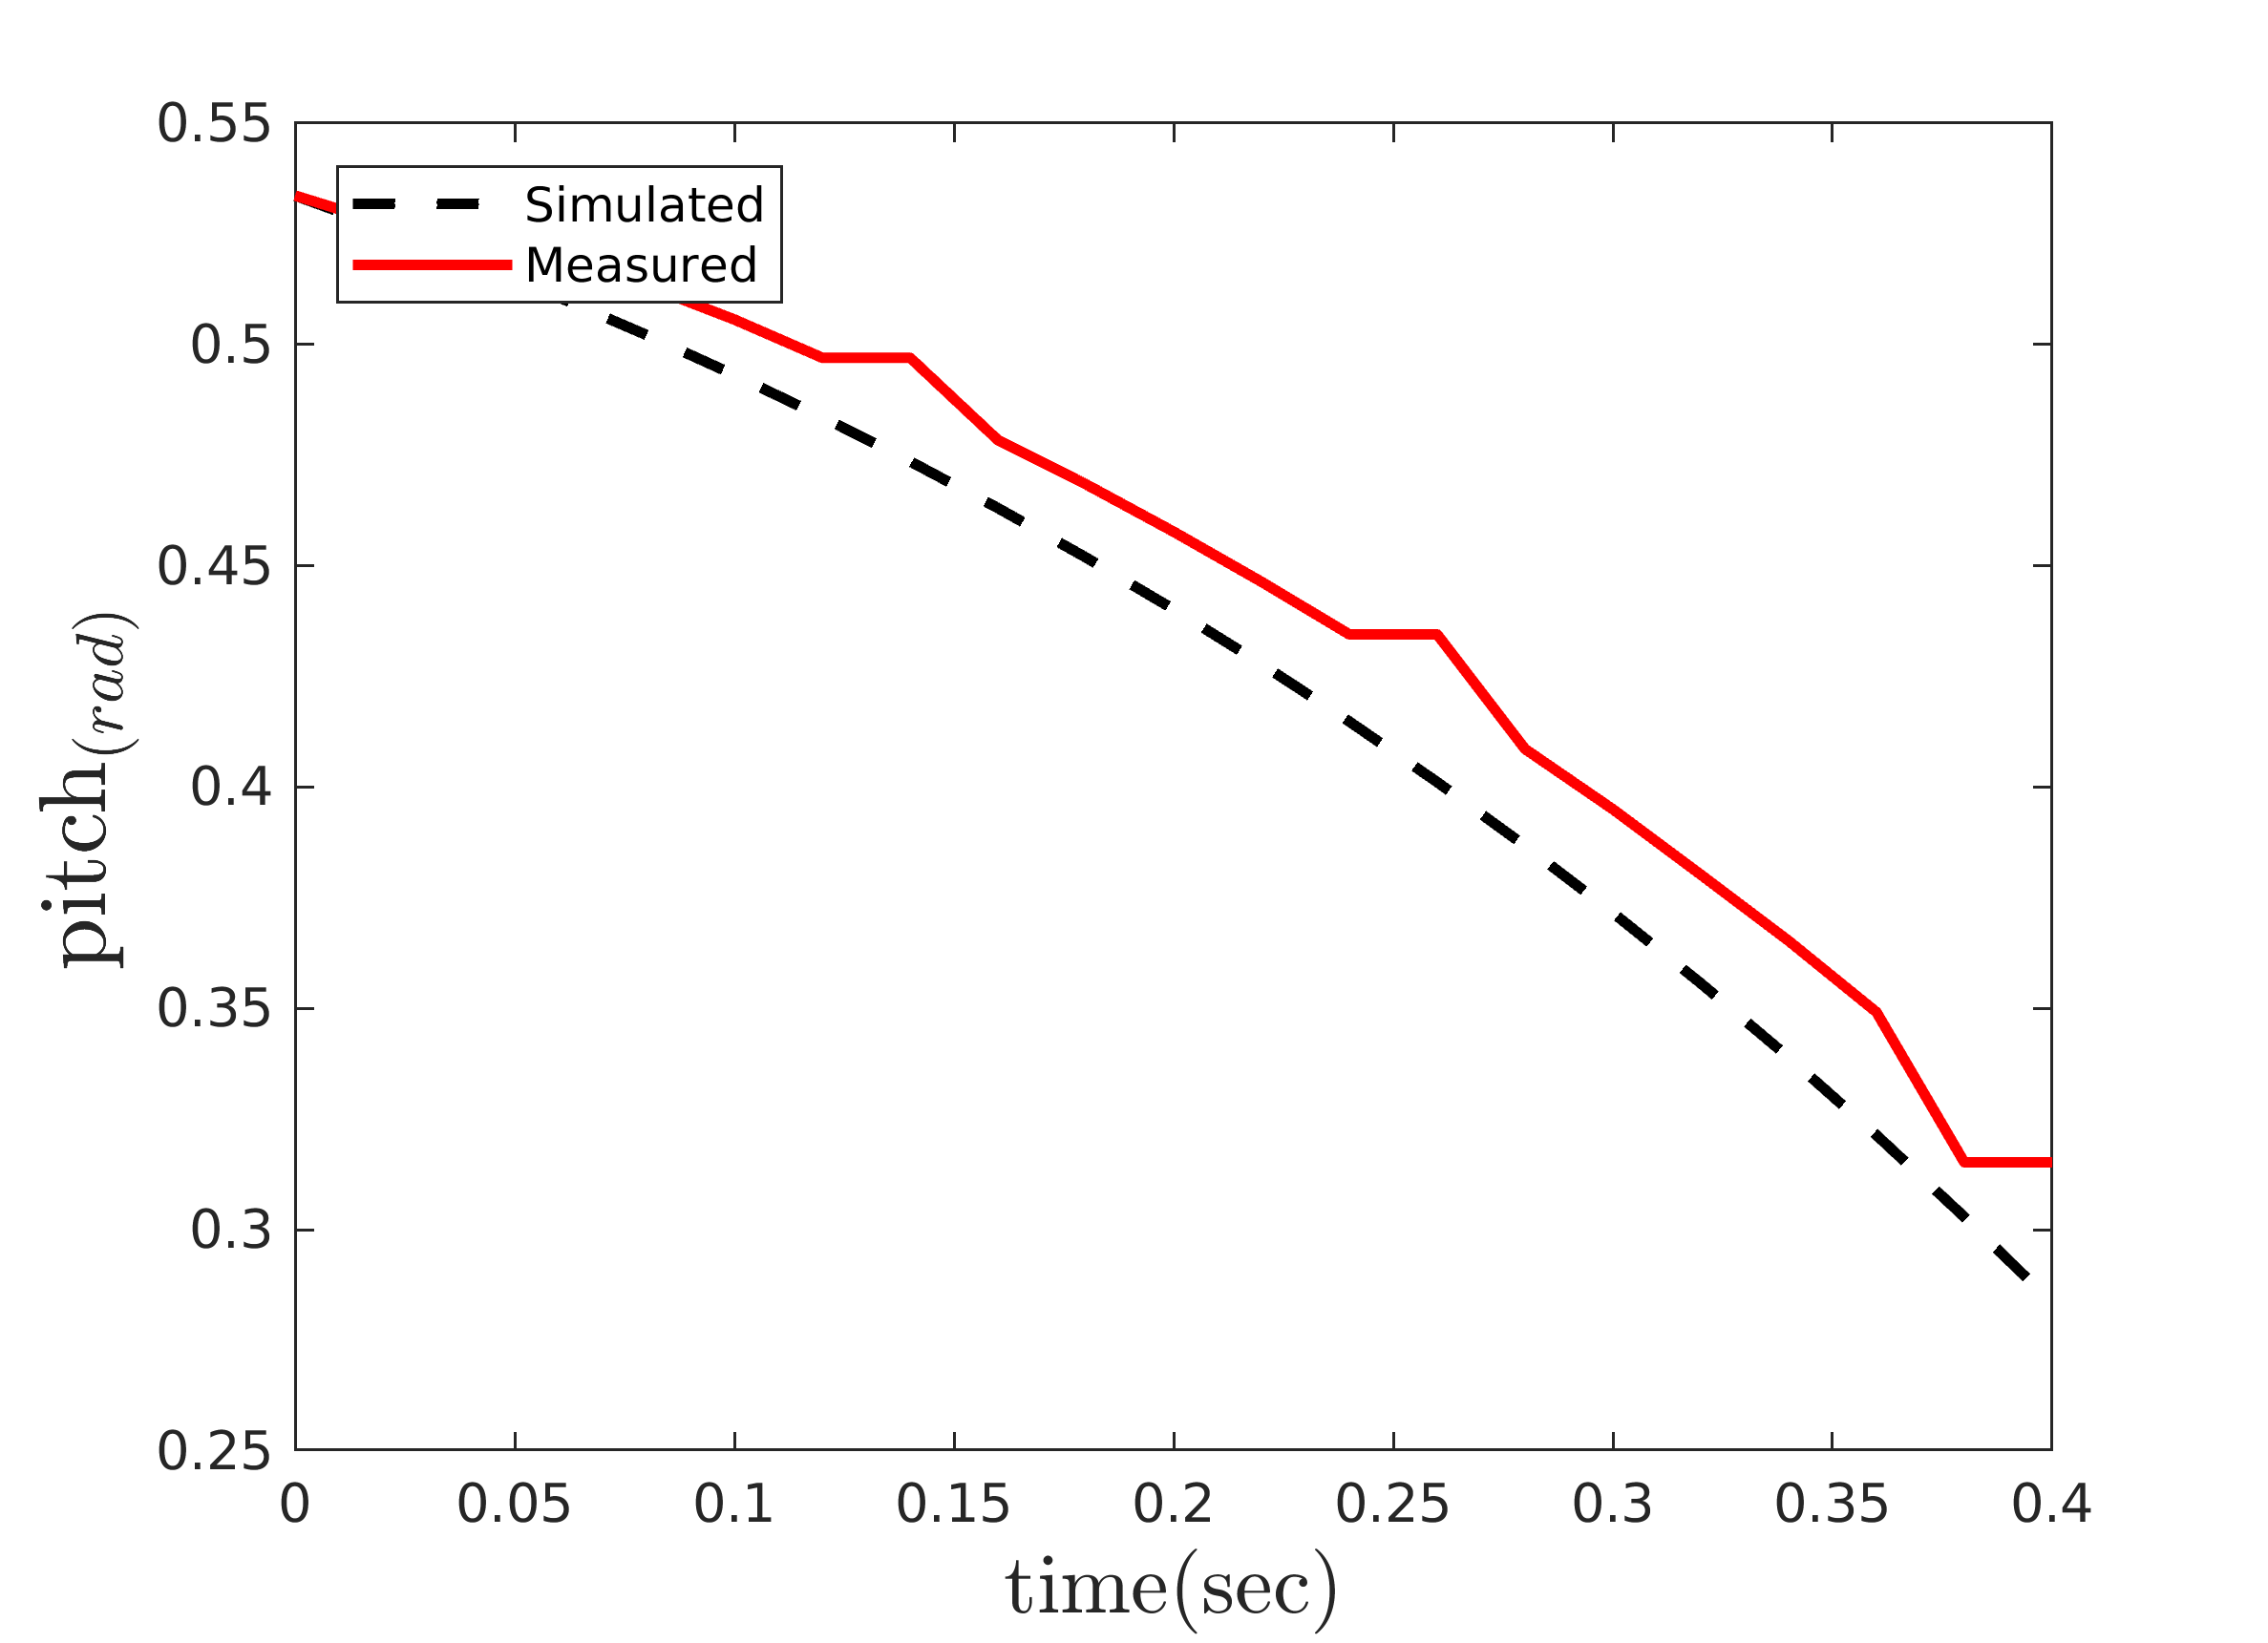
\includegraphics[width=12cm]{../Figures/RCP/pitch_ml_parameter_estimation/RCP_pitch_S4.png}
%	\centering
%	\caption{مقايسه وضعیت استند در  آزمايش چهارم و شبیه‌سازی، پس از تخمین پارامترهای کانال پیچ موتور خاموش}
%	\label{pitch_ml_ps4}
%\end{figure}
%\begin{figure}[H]
%	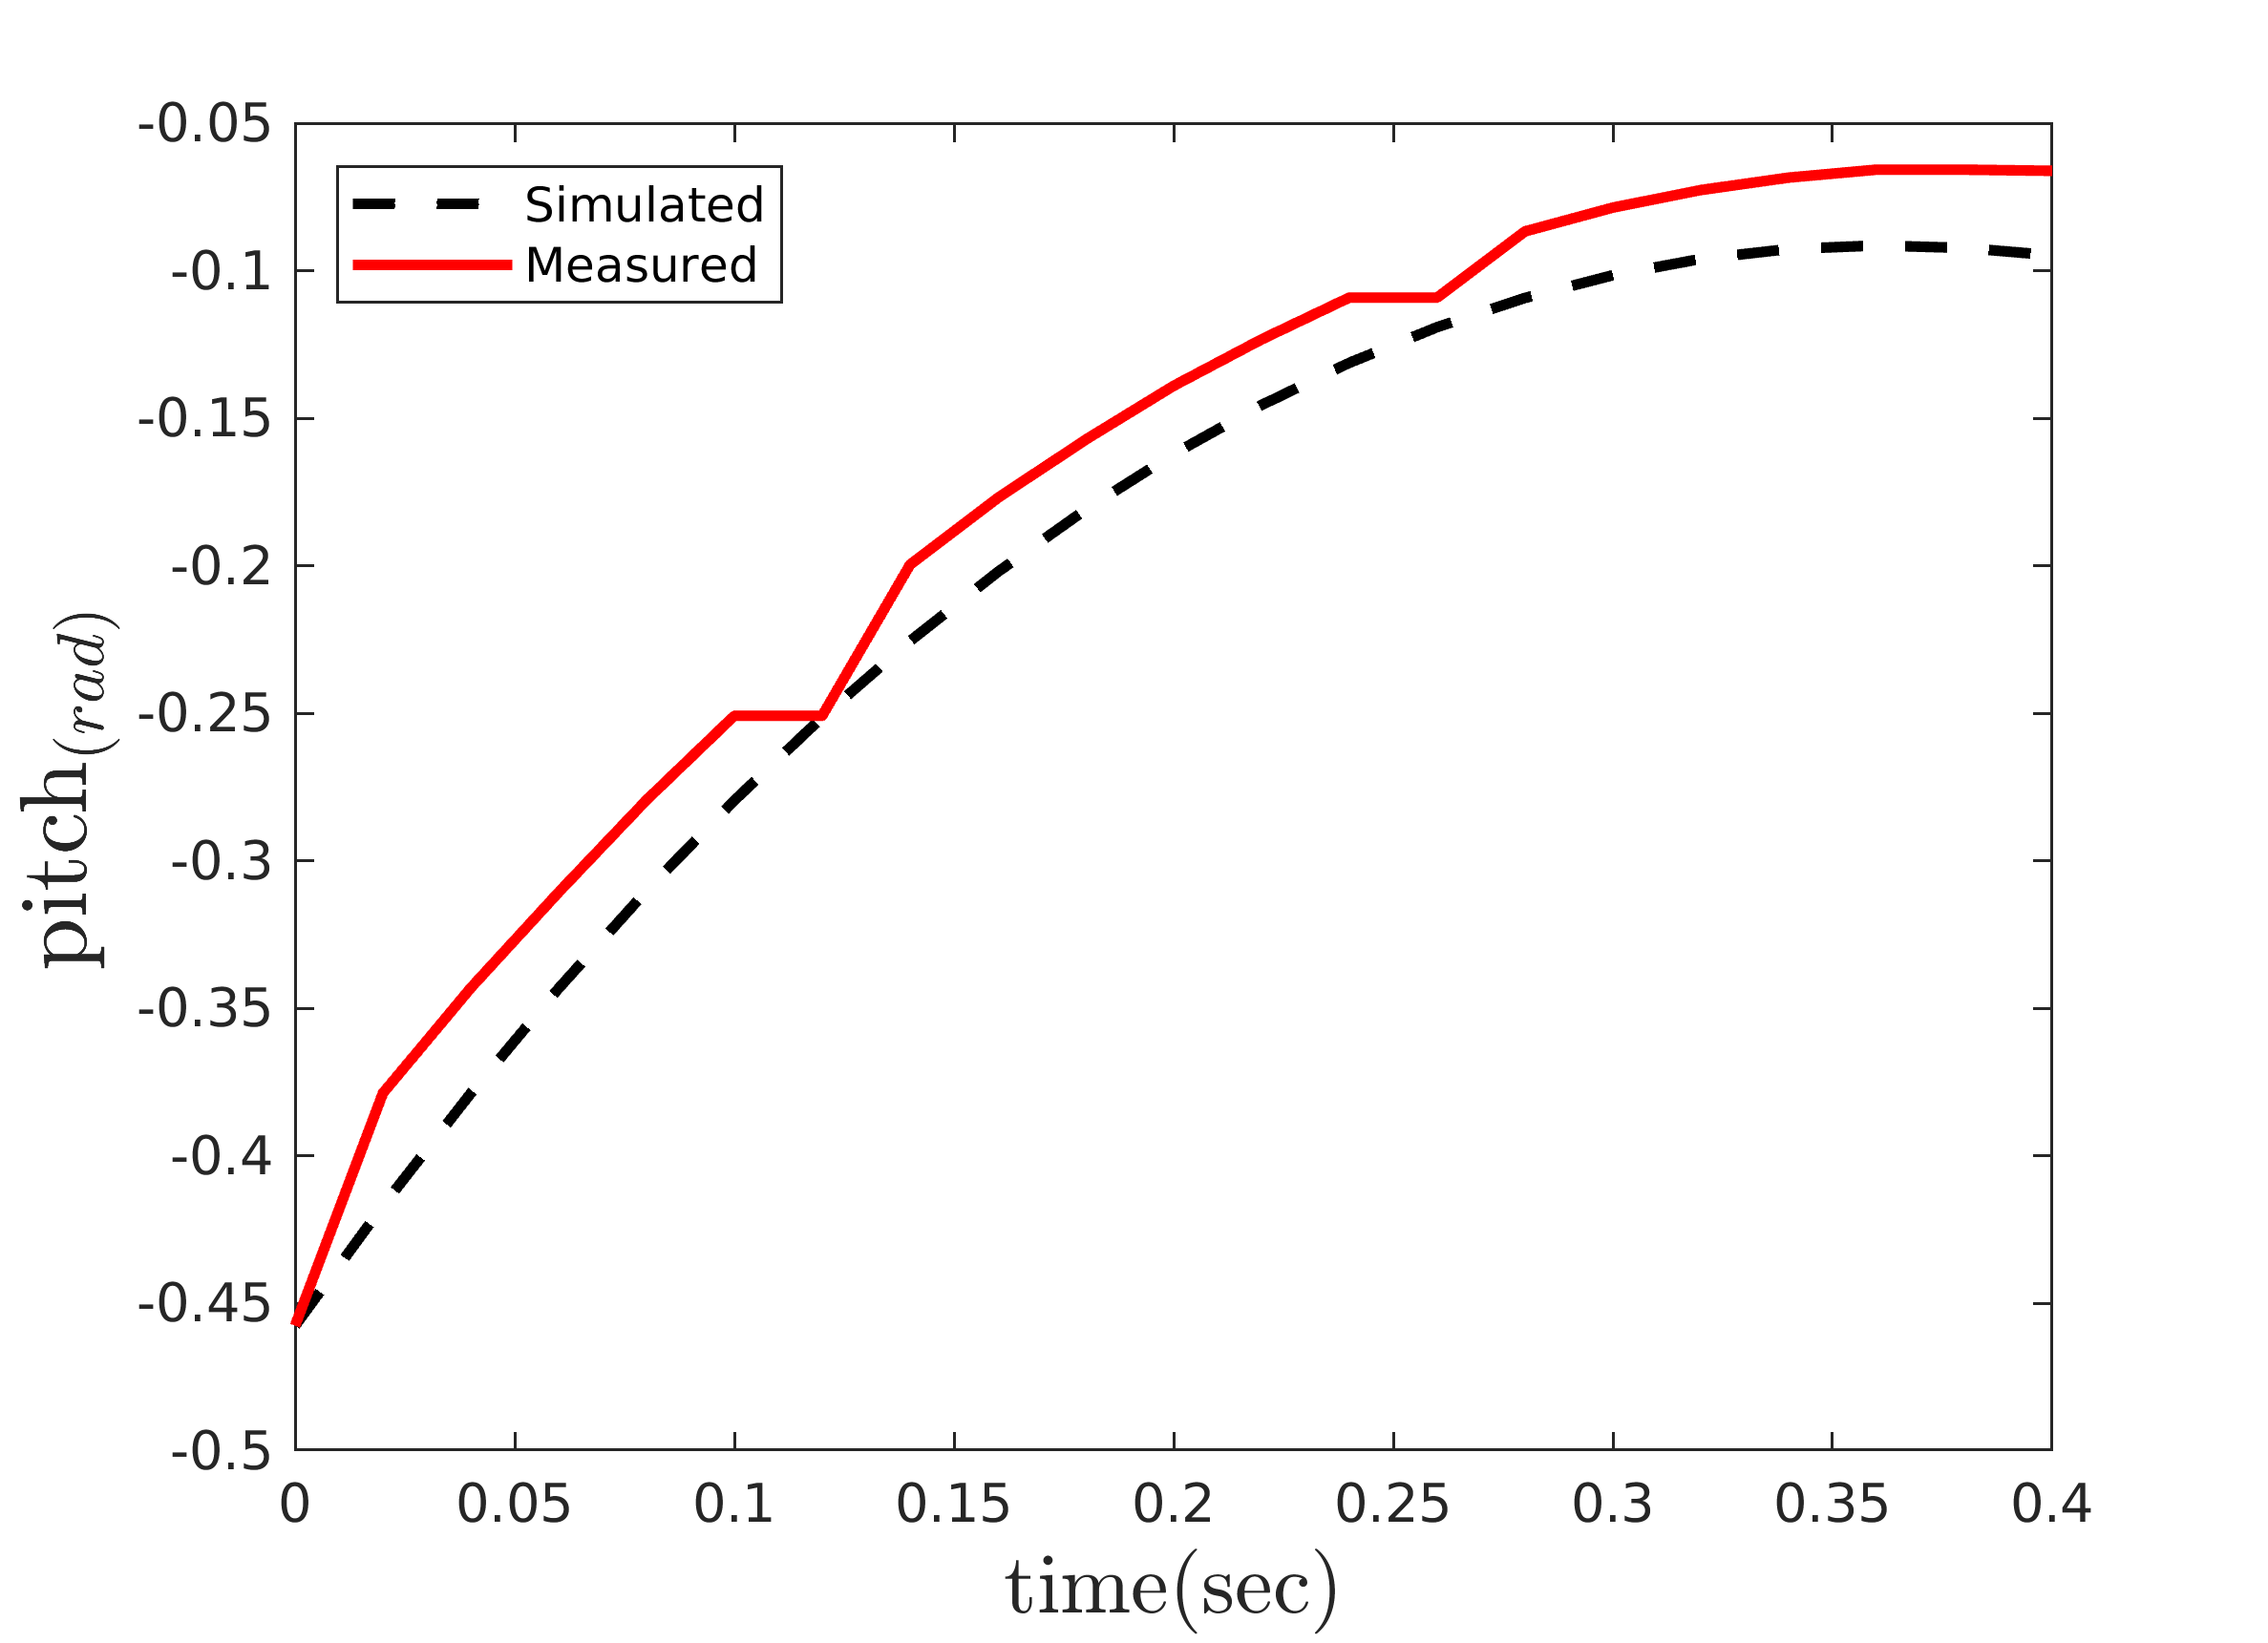
\includegraphics[width=12cm]{../Figures/RCP/pitch_ml_parameter_estimation/RCP_pitch_S5.png}
%	\centering
%	\caption{مقايسه وضعیت استند در  آزمايش پنجم و شبیه‌سازی، پس از تخمین پارامترهای کانال پیچ موتور خاموش}
%	\label{pitch_ml_ps5}
%\end{figure}
در ابتدا خروجی اصلاح پارامترهای کانال پیچ  حالت موتور خاموش و سپس حالت کلی آورده شده‌است.

  \begin{minipage}[H]{\linewidth}
	\hfill
	\begin{minipage}[b]{0.49\linewidth}
		\centering
		\begin{tabular}{ccc}\hline
			پارامتر & مقدار اولیه  & مقدار بعد از اصلاح
			\\ \hline
			$B_1$  & $4.53$ & $4.36$ \\
			$B_5$ & $0.007$ & $0.012$\\
			$B_6$ & $4.13$ & $4.428$\\ \hline
			\\\\
		\end{tabular}
	\captionsetup{justification=centering}
		\captionof{table}{مقايسه پارامترهای کانال پیچ موتور خاموش قبل و بعد از اصلاح}
	\end{minipage}
	\begin{minipage}[b]{0.48\linewidth}
		\centering
		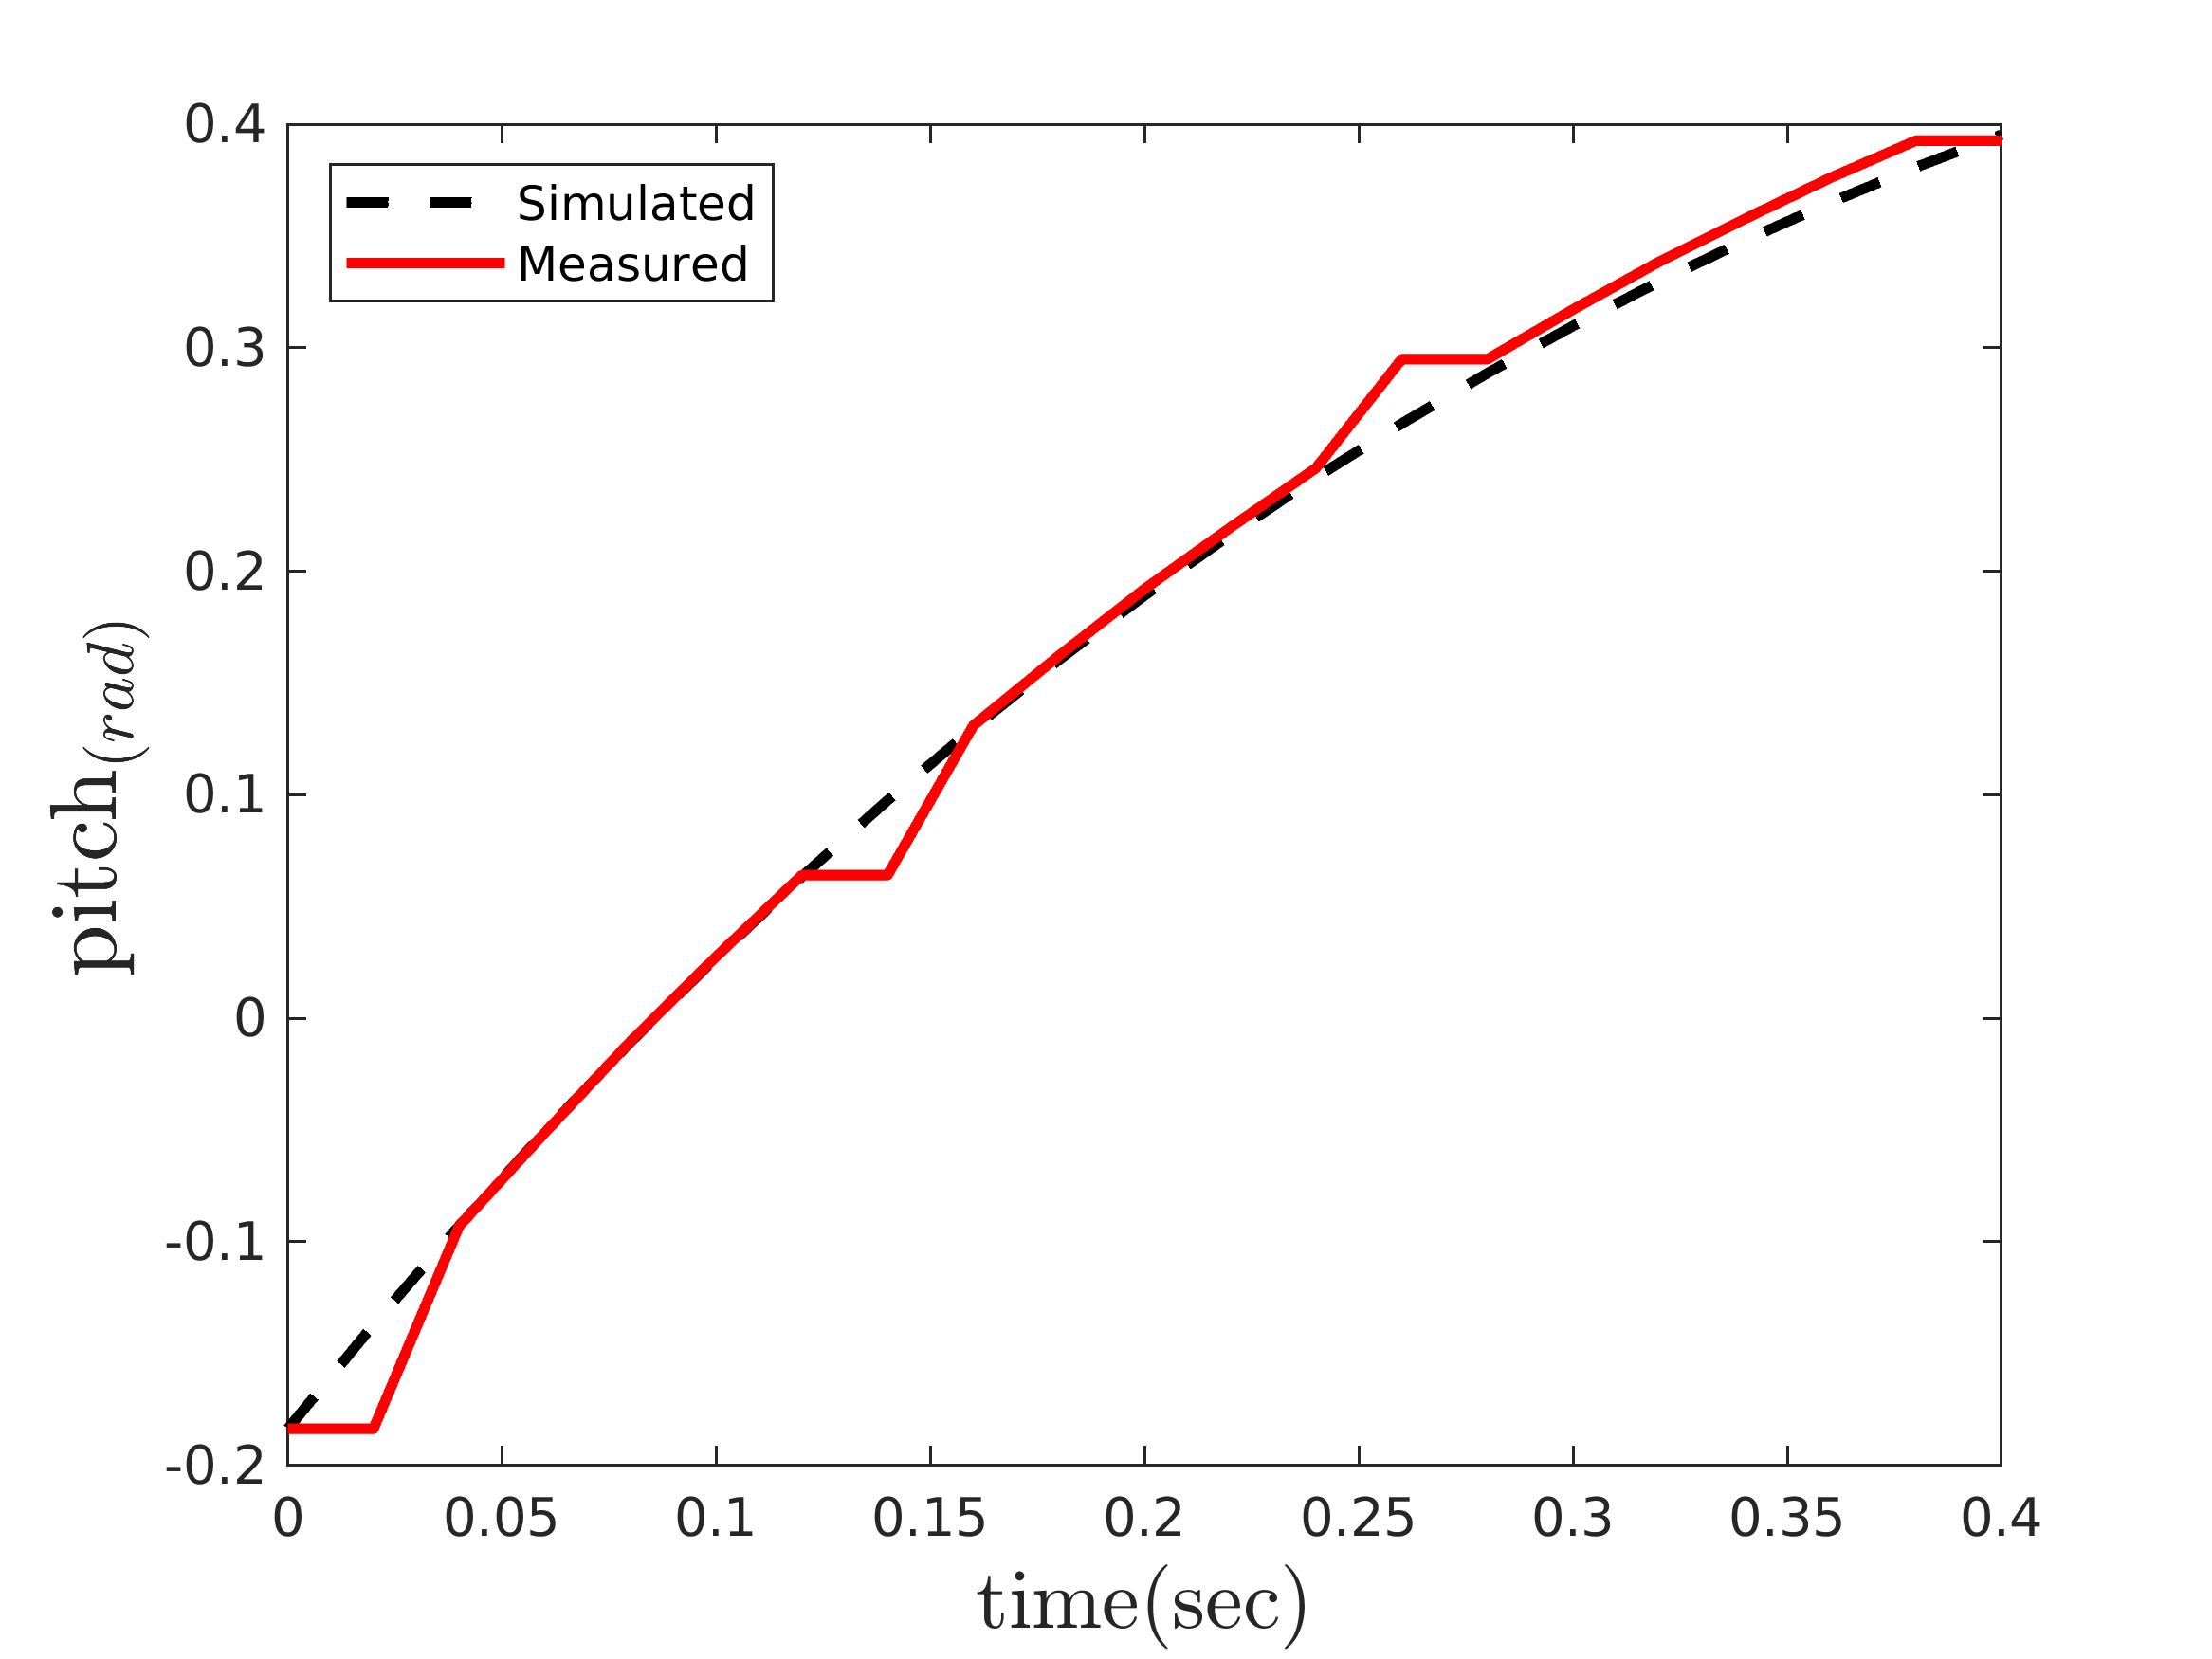
\includegraphics[width=1\linewidth]{../Figures/RCP/pitch_ml_parameter_estimation/RCP_pitch_S1.png}
		\captionsetup{justification=centering}
		\captionof{figure}{مقايسه وضعیت کانال پیچ موتور خاموش در شبیه‌سازی و واقعیت}
	\end{minipage}
\end{minipage}

